\chapter{Diffusion of innovation}
\label{chap:theory}

The researchers have studied the diffusion of innovation for a very long time. In the early 1940s, Bryce Ryan and Neal Gross~\cite{ryan1943diffusion} used the earlier sociological diffusion research~\cite{bowers1938differential}~\cite{chapin1928cultural} to show that the ideas of friends or the neighbors played an important role when an individual made the decision to adopt a new thing and they concluded that interpersonal channels were very important in the diffusion process. The diffusion of innovation theory is to study how, why and at what rate a new idea or product spreads through cultures. In the late 1950s and 1960s, the interest in studying the diffusion of innovation reached the peak and then declined. At that time, it was hard for the researchers to collect the data of the diffusion process and the usage of this theory was limited. In the past decades, with the development of the technology, people can conveniently communicate with each other through telephone and Internet, which has broken the geographical gap. Especially in recent years, the Internet technology has totally changed the way for people to acquire information. The appearance of the social media (e.g. blogs, email, and SNS) further allows everyone to express their own ideas which can also spread through the social media. This improvement has led to a resurgence of research on information diffusion and also made it much easier for the researcher to study all the users' behaviors which had been recorded and saved.   

In this chapter, first we will summarize the main idea of the diffusion of innovation theory and then we will review some diffusion applications.

\section{Diffusion of innovation theory}

\begin{figure}[!htb]
  \centering
  \includegraphics[width=300px]{figures/diffusionofideas.eps}
  \caption{The diffusion of innovation. With successive groups of consumers adopting the new technology (shown in blue), its market share (yellow) will eventually reach the saturation level. ~\cite{rogers1995diffusion}}
  \label{fig:diffusionofidea}
\end{figure}

The concept of the diffusion of innovation was first studied by Gabriel Tarde. After that, its basic epidemiological or internal-influence form was formulated by H. Earl Pemberton ~\cite{pemberton1936curve}, who provided examples of institutional diffusion such as postage stamps and compulsory school laws. In 1962, Rogers synthesized research from over 508 diffusion studies and proposed a theory for the adoption of innovations among individuals and organizations~\cite{rogers1995diffusion}. He identified 4 main elements in the process of the diffusion of innovation: the innovation, the communication channels, the time, and the social system. Combining these 4 elements, we can know that it is the process by which an innovation is communicated through certain channels over time among the members of a social system. In addition, Rogers claimed that there are 5 stages in the process of the diffusion of innovation: knowledge, persuasion, decision, implementation, and confirmation. Throughout the diffusion process there is evidence that not all individuals exert an equal amount of influence over all individuals. In this sense there are ``Opinion Leaders''~\cite{katz1955personal}(See Figure~\ref{fig:tsf}), who are influential in spreading either positive or negative information about an innovation. Rogers relied on the ideas of Katz & Lazarsfeld and the two-step flow theory in developing his ideas on the influence of opinion leaders in the diffusion process. Opinion leaders have the most influence during the evaluation stage of the innovation-decision process and over late adopters. In addition opinion leaders have a set of characteristics that set them apart from their followers and other individuals.

\begin{figure}[!htb]
  \centering
  \includegraphics{figures/twostepflow.eps}
  \caption{The schematic of the two-step flow model of influence ~\cite{watts2007influentials}. A small minority of ``opinion % leaders" (stars) act as intermediaries between the mass media and the majority of society (circles).}
  \label{fig:tsf}
\end{figure}

\section{Applications}
The diffusion of innovation theory has applications in a variety of fields. We will briefly discuss two applications: Viral marketing and public health.
\begin{itemize}

\item {Viral marketing}

\begin{figure}[!htb]
  \centering
  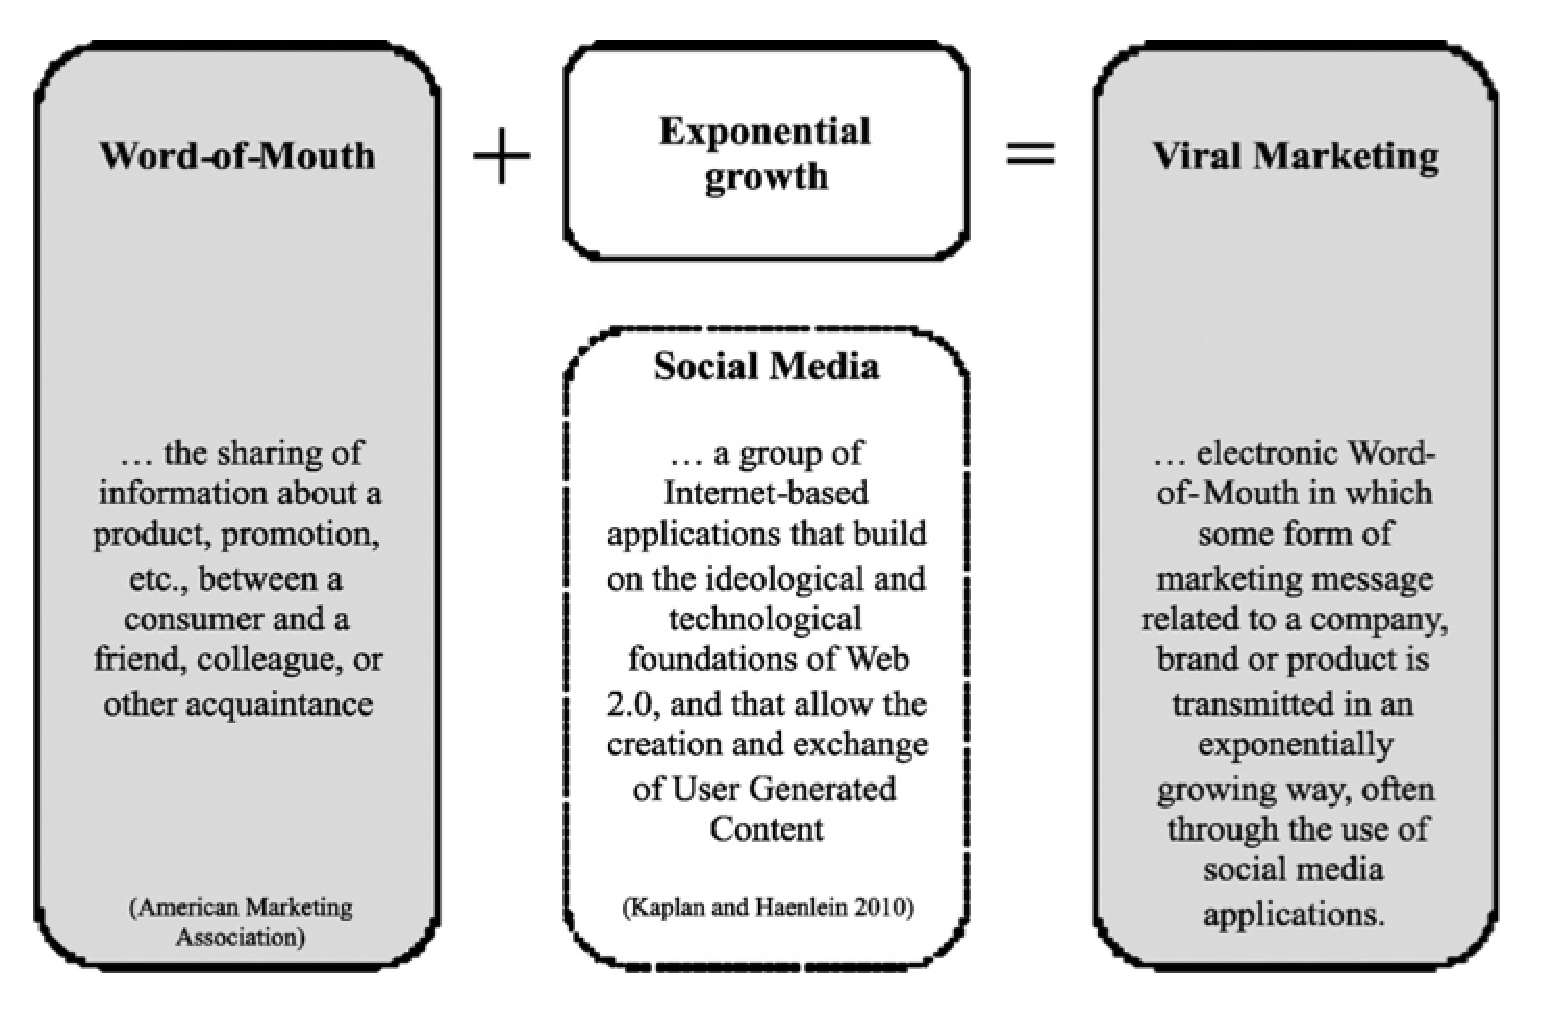
\includegraphics[width=400px]{figures/viralmarketing.eps}
  \caption{The relationship between word-of-mouth and viral marketing ~\cite{kaplan2011two}}
  \label{fig:relationwm}
\end{figure}

The viral marketing is the marketing technique that uses the pre-existing social network to achieve the marketing objectives like enhancing the brand awareness and increasing the product sales. The process of this kind of marketing is just like the virus spreading, which is self-replicating. The viral marketing can be delivered by word of mouth (WOM) and be enhanced by the network effects of Internet. 

From Fig.~\ref{fig:relationwm}, we can know the relationship between word-of-mouth and viral marketing as well as the roles they play. 
 
To make viral marketing work, we should meet three basic criteria:  the right people need to get the right message under the right circumstances~\cite{kaplan2011two}

One unique thing we should consider when analyzing the viral marketing is the marketing campaign. Just like any other marketing action, the campaign is also a very important factor which will affect the diffusion result through the social network.

\item Public health

Public health is "the science and art of preventing disease, prolonging life and promoting health through the organized efforts and informed choices of society, organizations, public and private, communities and individuals"~\cite{winslow1920untilled}. In~\cite{moore2004characteristics}, Moore claimed that the opinion leaders could provide an important vehicle for dissemination and adoption of evidence-based treatment practices in community treatment settings. Also, in~\cite{doumit2007local}, Doumit assesed the effectiveness of the use of local opinion leaders in improving the behavior of health care professionals and patient outcomes. 

Another topic in public health is how to control the spread of epidemic disease. In 1927, Kermack et al. created a model for the spreading of epidemic model called SIR model (See Chapter 4). This model is widely used and some concepts of the model have been adopted in other models. Newman used this model for a case of an epidemic in a structured polulation and confirmed the correctness of the exact solutions~\cite{newman2002spread}.

\end{itemize}
